\documentclass[tikz,border=4pt]{standalone}
\usepackage{tikz}
\usetikzlibrary{arrows.meta,positioning,fit,backgrounds}
\tikzset{
  block/.style={draw, rounded corners=2pt, align=center, text width=37mm, minimum height=9mm, inner sep=3pt, font=\small\sffamily},
  smallblock/.style={draw, rounded corners=2pt, align=center, text width=32mm, minimum height=8mm, inner sep=3pt, font=\small\sffamily},
  flow/.style={-Latex, semithick},
  groupbox/.style={draw, rounded corners=3pt, inner sep=6pt},
  grouplabel/.style={font=\bfseries\small\sffamily, anchor=south west}
}
\begin{document}
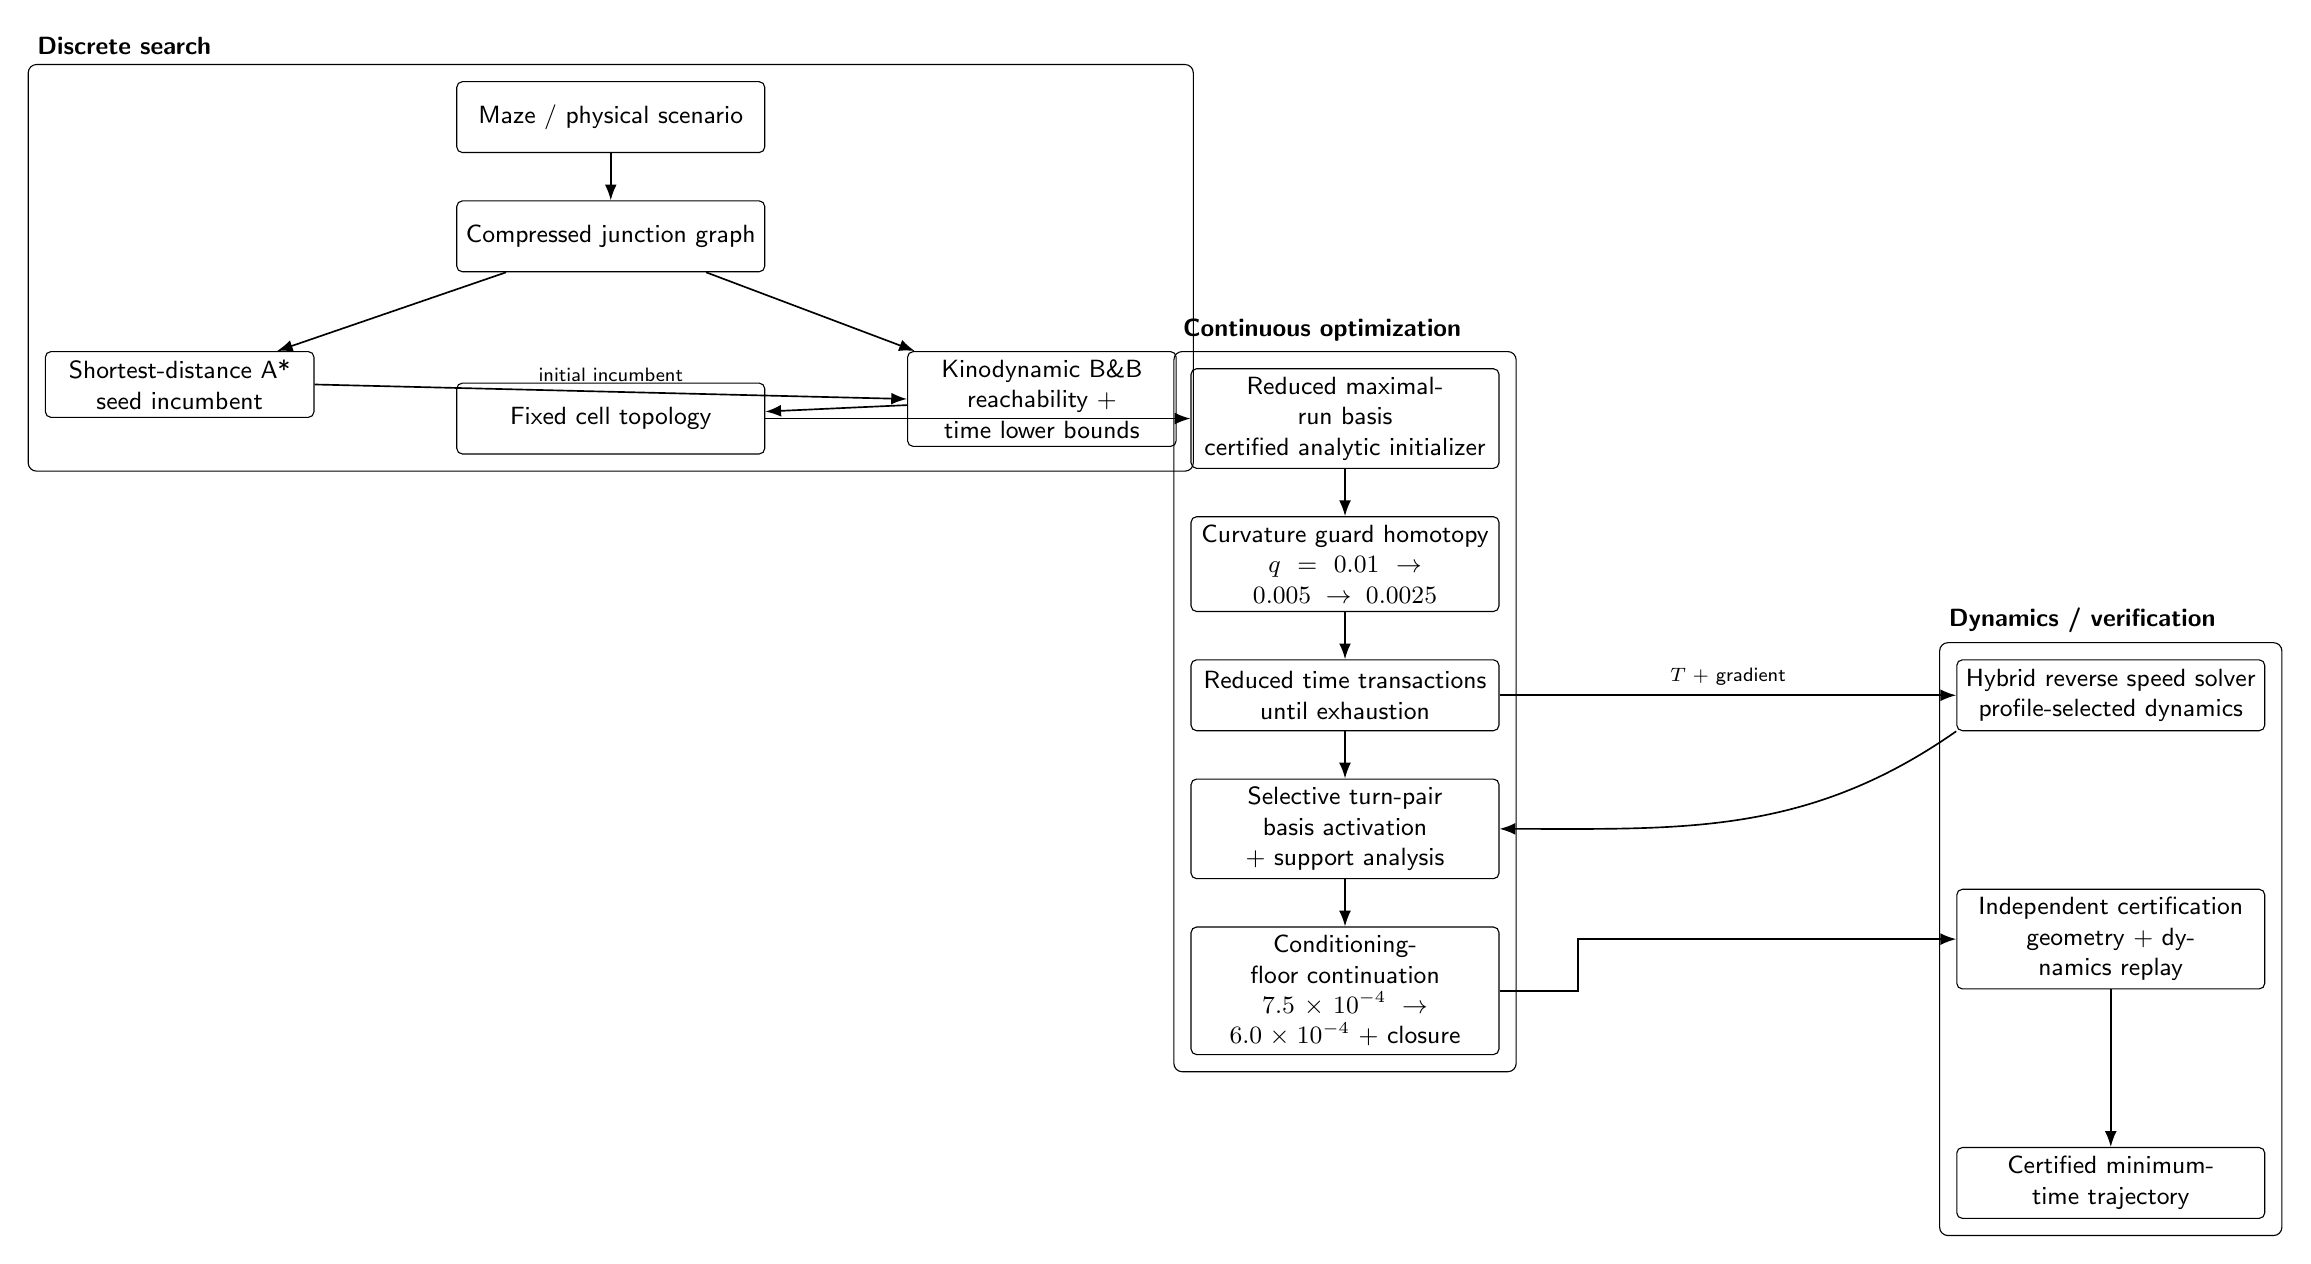
\begin{tikzpicture}[node distance=6mm and 12mm]
  % Discrete search
  \node[block] (maze) at (0,0) {Maze / physical scenario};
  \node[block, below=of maze] (graph) {Compressed junction graph};
  \node[smallblock, below left=10mm and 18mm of graph] (astar) {Shortest-distance A*\\seed incumbent};
  \node[smallblock, below right=10mm and 18mm of graph] (bnb) {Kinodynamic B\&B\\reachability + time lower bounds};
  \node[block, below=14mm of graph] (topology) {Fixed cell topology};

  % Continuous optimization
  \node[block, right=54mm of topology] (reduced) {Reduced maximal-run basis\\certified analytic initializer};
  \node[block, below=of reduced] (curv) {Curvature guard homotopy\\$q=0.01 \rightarrow 0.005 \rightarrow 0.0025$};
  \node[block, below=of curv] (time) {Reduced time transactions\\until exhaustion};
  \node[block, below=of time] (basis) {Selective turn-pair basis activation\\+ support analysis};
  \node[block, below=of basis] (floor) {Conditioning-floor continuation\\$7.5\times10^{-4} \rightarrow 6.0\times10^{-4}$ + closure};

  % Dynamics / verification
  \node[block, right=58mm of time] (speed) {Hybrid reverse speed solver\\profile-selected dynamics};
  \node[block, below=20mm of speed] (cert) {Independent certification\\geometry + dynamics replay};
  \node[block, below=20mm of cert] (out) {Certified minimum-time trajectory};

  % Flows
  \draw[flow] (maze) -- (graph);
  \draw[flow] (graph) -- (astar);
  \draw[flow] (graph) -- (bnb);
  \draw[flow] (astar.east) -- node[above, font=\scriptsize\sffamily] {initial incumbent} (bnb.west);
  \draw[flow] (bnb) -- (topology);
  \draw[flow] (topology) -- (reduced);
  \draw[flow] (reduced) -- (curv);
  \draw[flow] (curv) -- (time);
  \draw[flow] (time) -- (basis);
  \draw[flow] (basis) -- (floor);
  \draw[flow] (time.east) -- node[above, font=\scriptsize\sffamily] {$T$ + gradient} (speed.west);
  \draw[flow] (speed.south west) to[out=-145,in=0] (basis.east);
  \draw[flow] (floor.east) -- ++(10mm,0) |- (cert.west);
  \draw[flow] (cert) -- (out);

  % Group boxes
  \begin{scope}[on background layer]
    \node[groupbox, fit=(maze)(graph)(astar)(bnb)(topology)] (g1) {};
    \node[grouplabel] at (g1.north west) {Discrete search};
    \node[groupbox, fit=(reduced)(curv)(time)(basis)(floor)] (g2) {};
    \node[grouplabel] at (g2.north west) {Continuous optimization};
    \node[groupbox, fit=(speed)(cert)(out)] (g3) {};
    \node[grouplabel] at (g3.north west) {Dynamics / verification};
  \end{scope}
\end{tikzpicture}
\end{document}
